\documentclass[12pt]{article}
%Gummi|065|=)
\usepackage[a4paper,margin=2.5cm]{geometry}
\usepackage{float}
\usepackage{graphicx}
\usepackage{pdfpages}
\title{\textbf{PPRO0605 - Rapport de projet}}
\author{
		BAKALI-HEMOU Yempabe\\
		FRANZ Raphaël\\
		MIRGAINE Paul
		}
\date{}

\renewcommand{\contentsname}{Sommaire}

\begin{document}


\includepdf{page_garde.pdf}

\section*{Introduction}

Pour la matière PPRO0605, il nous a été demandé de réalisée une application web de gestion des LANs pour la fac. L'application doit être réalisée en PHP et plus précisément, avec le framework Laravel vu en INFO0303. MySql a été utilisé pour la gestion de la base de données. Dans un premier temps, ce rapport se penchera sur la partie conception de l'application, puis il abordera notre organisation avant de passer à une présentation de l'application.
\tableofcontents

\newpage

\section{Conception et analyse}
La première tâche a été d'effectuer la conception de l'application pour mieux cerner le sujet, se mettre d'accord sur le sens de certains éléments et avoir notre base pour commencer le développement. La première analyse effectuée est un diagramme de cas d'utilisation, qui nous a permis de se mettre d'accord sur les acteurs de l'application et les actions nécessaires. Puis la réalisation du diagramme de navigation nous permet d'obtenir les relations entre les pages et aussi la liste des vues qu'il sera nécessaire de réaliser. En parallèle nous avons fait l'étude de la base de données à l'aide d'un MCD décrit dans la troisième partie.
\subsection{Cas d'utilisation}

Nous avons identifié trois profils d'utilisateurs dans notre application. Tout d'abord les visiteurs qui ont, de plus que la page d'accueil, accès à la liste des LANs. De plus un visiteur peut se connecter ou s'inscrire. 
\newline

Le deuxième type de profil est l'utilisateur, qui peut en plus de voir les LANs, il peut s'y inscrire. Il peut s'inscrire comme joueur ou se proposer pour aider l'organisation. Dans ce cas, il peut possiblement voir les tâches que l'organisation lui donne. 
\newline

Finalement, le dernier profil est celui de l'organisateur, qui peut accéder à la page de gestion des LANs. Il peut décider de créer une LAN, d'en supprimer ou d'en modifier une ou de la publier pour qu'elles apparaissent dans la liste publique et que les utilisateurs puissent la rejoindre.
\newline

En faisant la synthèse des éléments cités précédemment, on obtient le diagramme des cas d'utilisation suivant :

\begin{figure}[H]
\centering
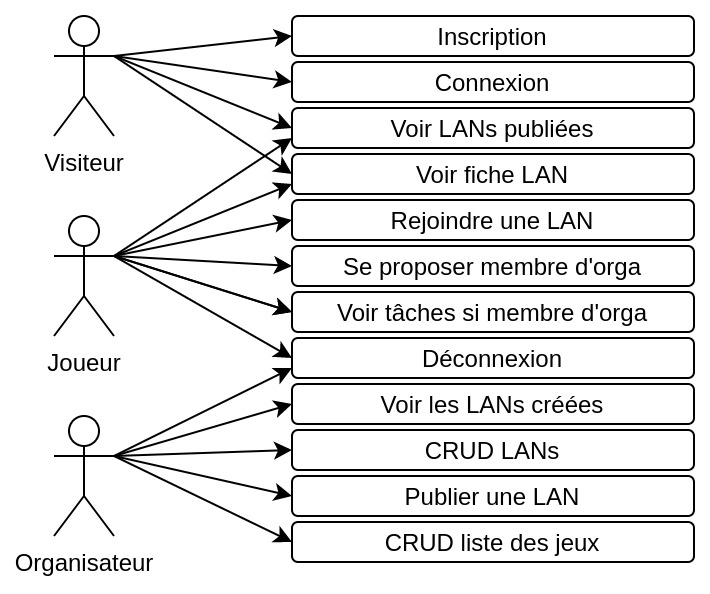
\includegraphics[scale=.40]{images/cas_utilisation.jpg}
\caption{Diagramme des cas d'utilisations}
\label{}
\end{figure}

\subsection{Diagramme de navigation}
\begin{figure}[H]
\centering
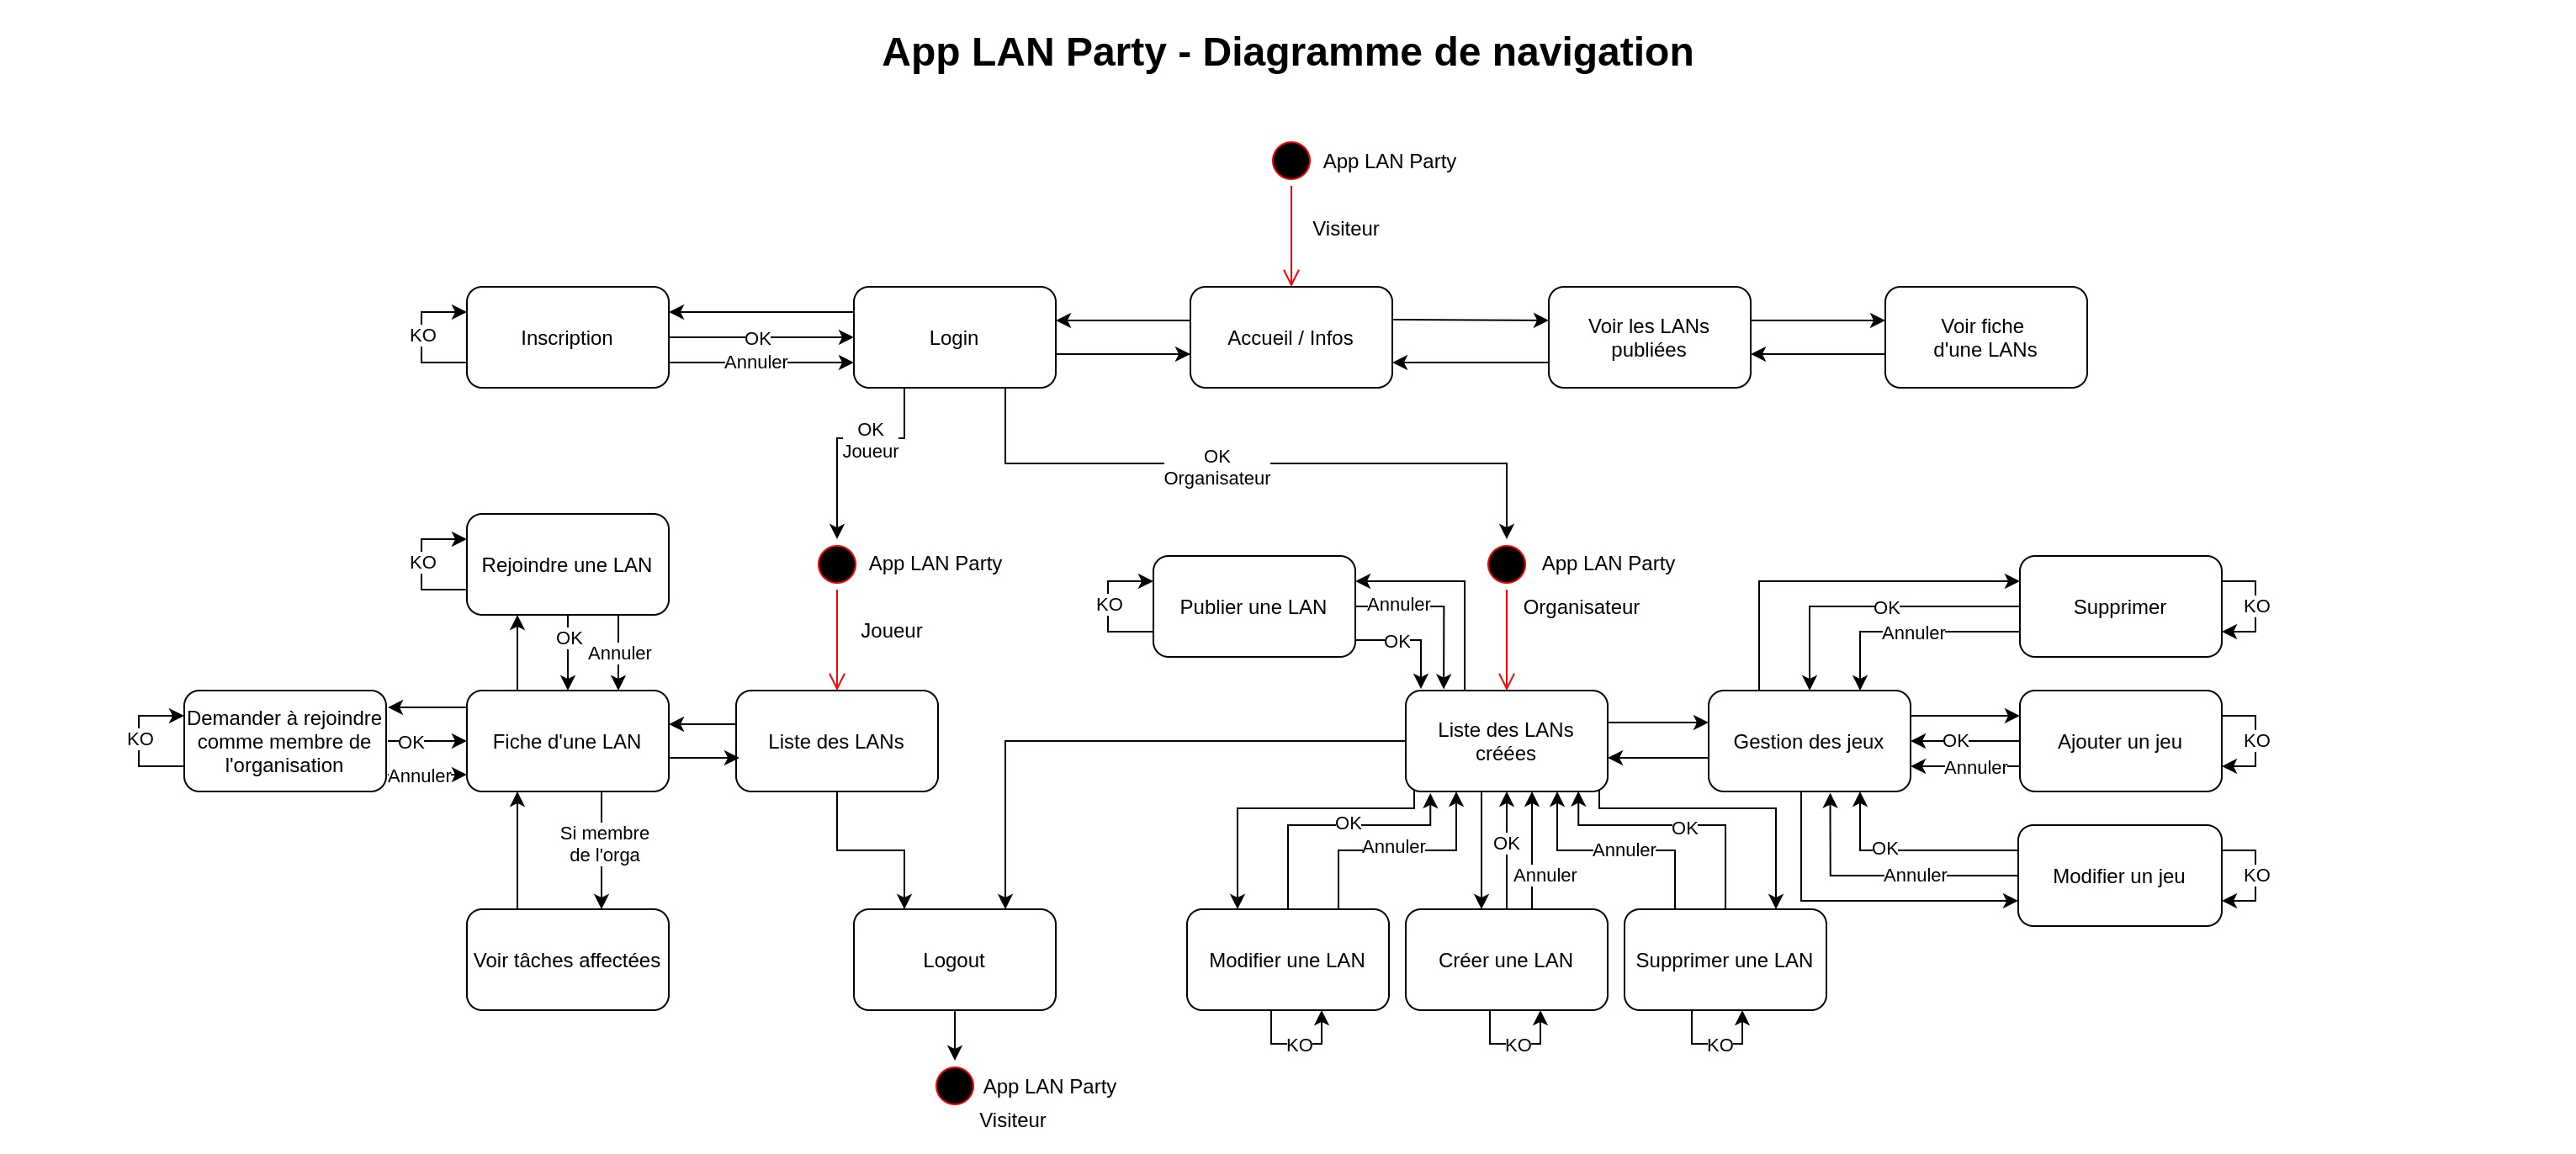
\includegraphics[scale=0.21,angle=90,origin=c]{images/navigation.jpg}
\caption{Diagramme de navigation}
\label{}
\end{figure}


Le site sera donc composé de trois parties, la partie commune à tous les utilisateurs, la partie accessible par les joueur et celle uniquement accessible par les organisateur.
\newline

Dans la partie commune on retrouve donc la page d'accueil, le système d'inscription/connexion et la liste des LANs publiées dans lesquelles on peut naviguer librement. 
\newline

Lorsque l'on se connecte en tant que joueur, on peut accéder à la liste des LANs mais avec la possibilité d'en rejoindre une. De plus si le joueur se propose comme membre d'organisation, il peut accéder aux tâches que les organisateur auraient pu leur donner. 
\newline

Finalement, un organisateur peut accéder à la liste des LANs publiées ou non, et faire toutes les actions possibles sur elles.
\newpage
\subsection{Analyse de la base de données}

Notre base de données se compose de deux parties principales : la première contient tous ce qui touche aux utilisateurs, le seconde tous ce qui touche aux LANs. 
\newline

Les utilisateurs ont leurs propres table, mais possèdent aussi une table permettant de modéliser les rôles (joueur ou organisateur), et une table correspondant aux tâches qui peuvent être attribués aux joueurs. 
\newline

Les LANs, en plus de leur table propre, possèdent des tables pour les tournois, les jeux, le matériel et les salles. 
\newline

Les liens entre ses deux grandes parties sont le fait que les joueurs s'inscrivent aux LANs.
\newline

Voici le MCD que nous avons conçu à partir de ses informations : 

\begin{figure}[htp]
\centering
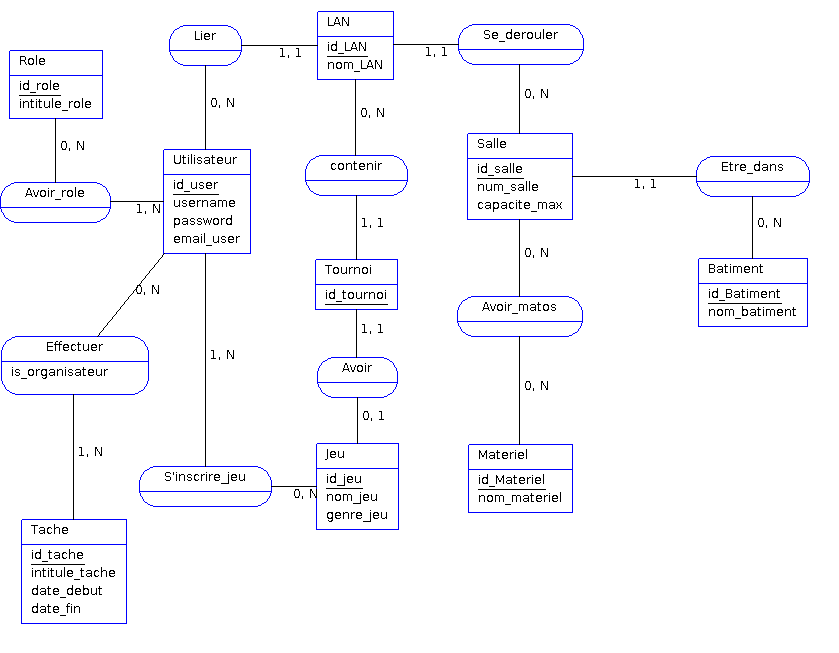
\includegraphics[scale=0.50]{images/mcd.png}
\caption{MCD de l'application}
\label{}
\end{figure}

\newpage

\section{Détoulement du développement}

\subsection{Organisation}

Bien évidemment, les circonstances actuelles ont eu un important impact sur l'organisation du travail. Nous avons donc organisé notre travail en conséquence car nous avons uniquement travaillé à distance sur le projet. Pour cela nous avons utilisé pour communiquer le programme Discord. Toutes les décisions ont été prise en ce consultant sur notre conversation. Nous avons privilégié la communication écrite car toutes les conditions n'étaient pas réunies pour organiser les conversations en vocale. Nous effectuions une mise au point tous les quelques jours et prévenons de nos avancements les autres membres du groupe. Pour le partage des sources nous avons utilisé Git et mis en ligne le repo sur GitHub.

\subsection{Partage du travail}

Nous avons tous d'abord avant de commencer le projet, chacun de notre côté, remis nos mains sur le framework
Laravel pour reprendre connaissances des différents concepts, leurs mises en place et les changements proposé par la sortie de la version 7 de Laravel.

Dû à la petite taille de notre équipe, nous avons décidé de partager le travail au fur et à mesure de notre progression. 

La première étape a donc été la phase de conception, décrite dans la première partie de ce rapport. Deux d'entre nous se sont occupé de l'analyse de la base de données pendant que le dernier a établit les cas d'utilisation et le diagramme  de navigation.

Par la suite, nous nous partagions le travail au fur et à mesure. Nous avons donc tous touché à tous les aspects de l'application mais pas sur les mêmes parties.

\subsection{Problèmes rencontrés et solutions}
\begin{itemize}
\item Problème de matériel (confinement)
\item Problème de fichiers entre IDE et Editeur classique (certains fichiers ne sont pas push) et problème de version du code (il faut gérer si plusieurs fichiers sont modifiés en même temps)
\item Installation de bibliothèques externes, compatibles avec Laravel 6 mais pas 7.x
\end{itemize}

\subsection{Acquis de chacun}

- Yempabe: Travailler en équipe réduite demande beaucoup plus d'efforts (et de temps), surtout lors de la condition actuelle. J'ai pu me remettre dans le bain de la programmation web. Et ce projet m'a donné envie d'approfondir mes connaissances dans ce domaine et me donner de nouveaux objectifs.


- Raphaël: J'ai pu redécouvrir le framework Laravel et corriger les erreurs apprises grâces aux précédents projets effectués sous Laravel en INFO0303. Cela m'a aussi permis de met remettre dans la programmation web et d'en redécouvrir les concepts. Mais même en ayant compris certaines choses que je ne comprenais pas avant, d'autres problématiques sont apparues, avec en premier lieu la redécouverte de Laravel 7 dont il faut réapprendre les concepts qui ont été changés avec la nouvelle version. Malgré les conditions difficiles et pas toujours idéales, ce projet m'a aussi appris à travailler à distance sur un projet à plusieurs, avec les problématiques associés.


- Paul: Comme mes collègues, le travail à distance avec une équipe de plus de deux personne est une nouveauté pour moi. Malheureusement, la situation actuelle et certains problèmes personnels ne m'ont pas permis de m'investir comme il se doit dans ce projet.
\newpage

\section{Présentation de l'application}

\subsection{Partie publique}
Lorsque l'on se connecte à l'application, nous atterrissons sur la page d'accueil. Sur celle-ci nous retrouvons un lien permettant d'accéder à la liste des LANs, ainsi que les liens pour les formulaires de connexion et d'inscription.

\begin{figure}[H]
\centering
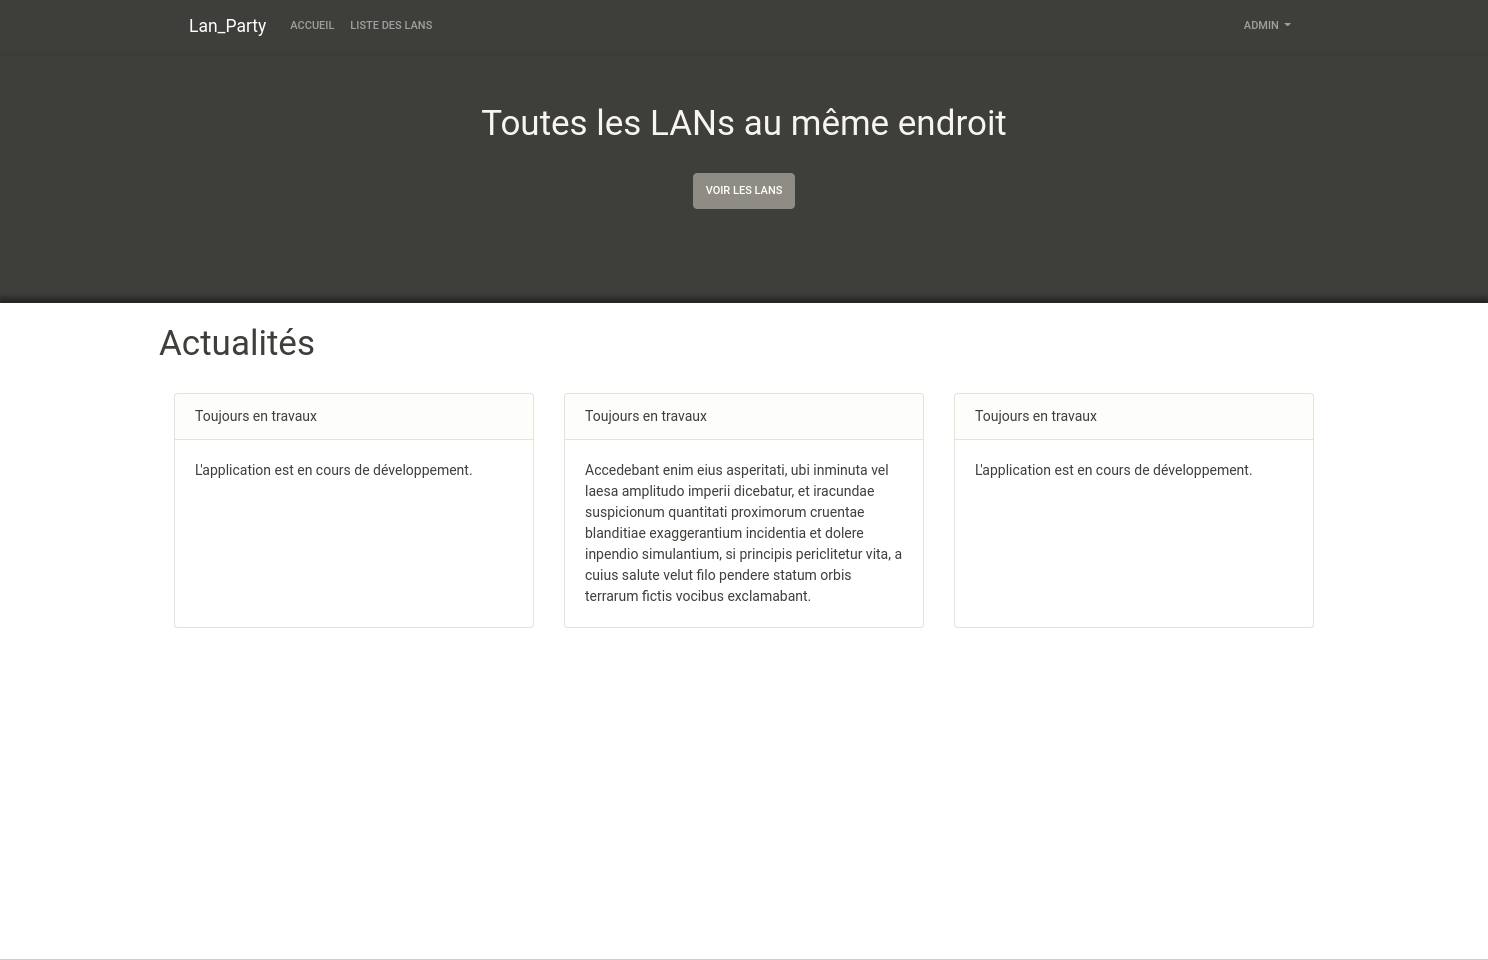
\includegraphics[scale=0.20]{images/accueil.png}
\caption{Page d'accueil}
\label{}
\end{figure}

\begin{figure}[H]
\centering
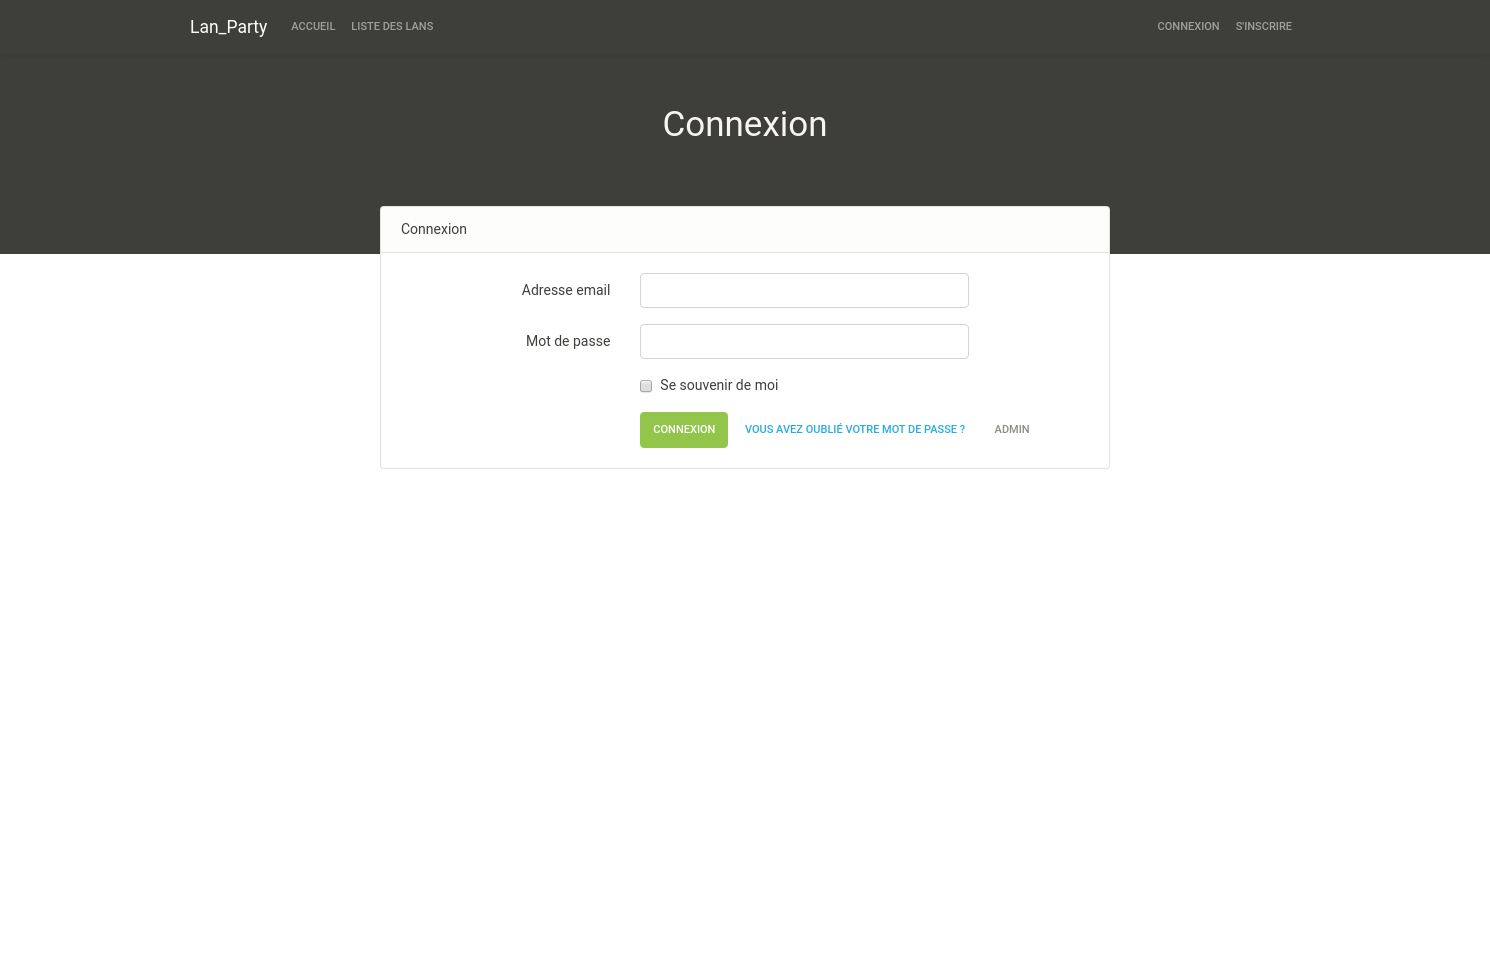
\includegraphics[scale=0.20]{images/connexion.jpg}
\caption{Page de connexion}
\label{}
\end{figure}

\begin{figure}[H]
\centering
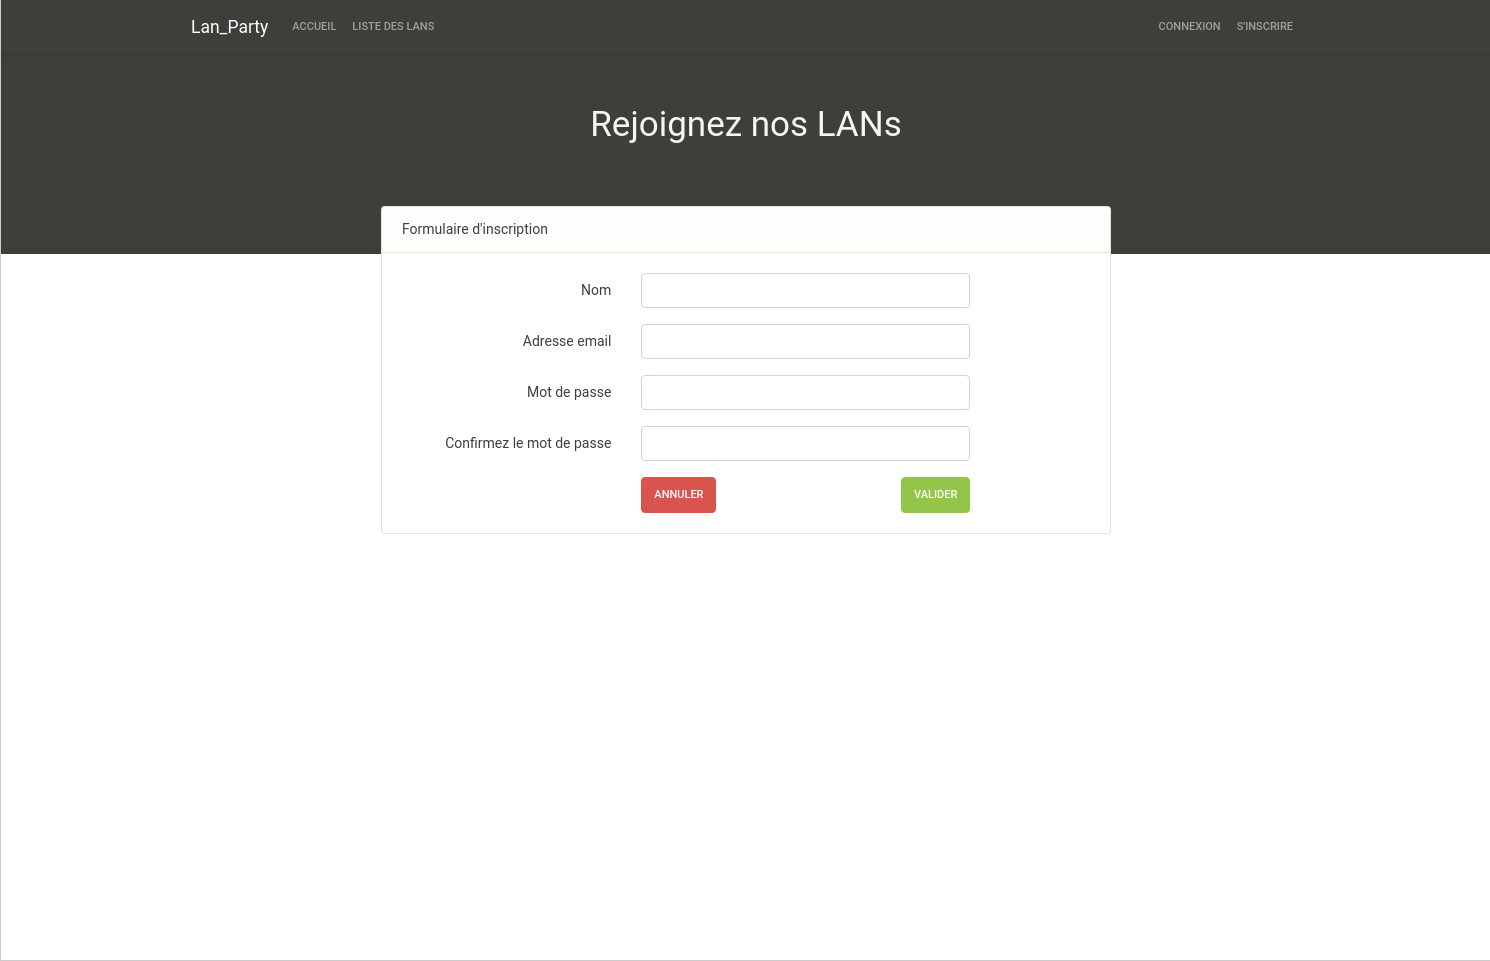
\includegraphics[scale=0.20]{images/inscription.png}
\caption{Page d'inscription}
\label{}
\end{figure}

\begin{figure}[H]
\centering
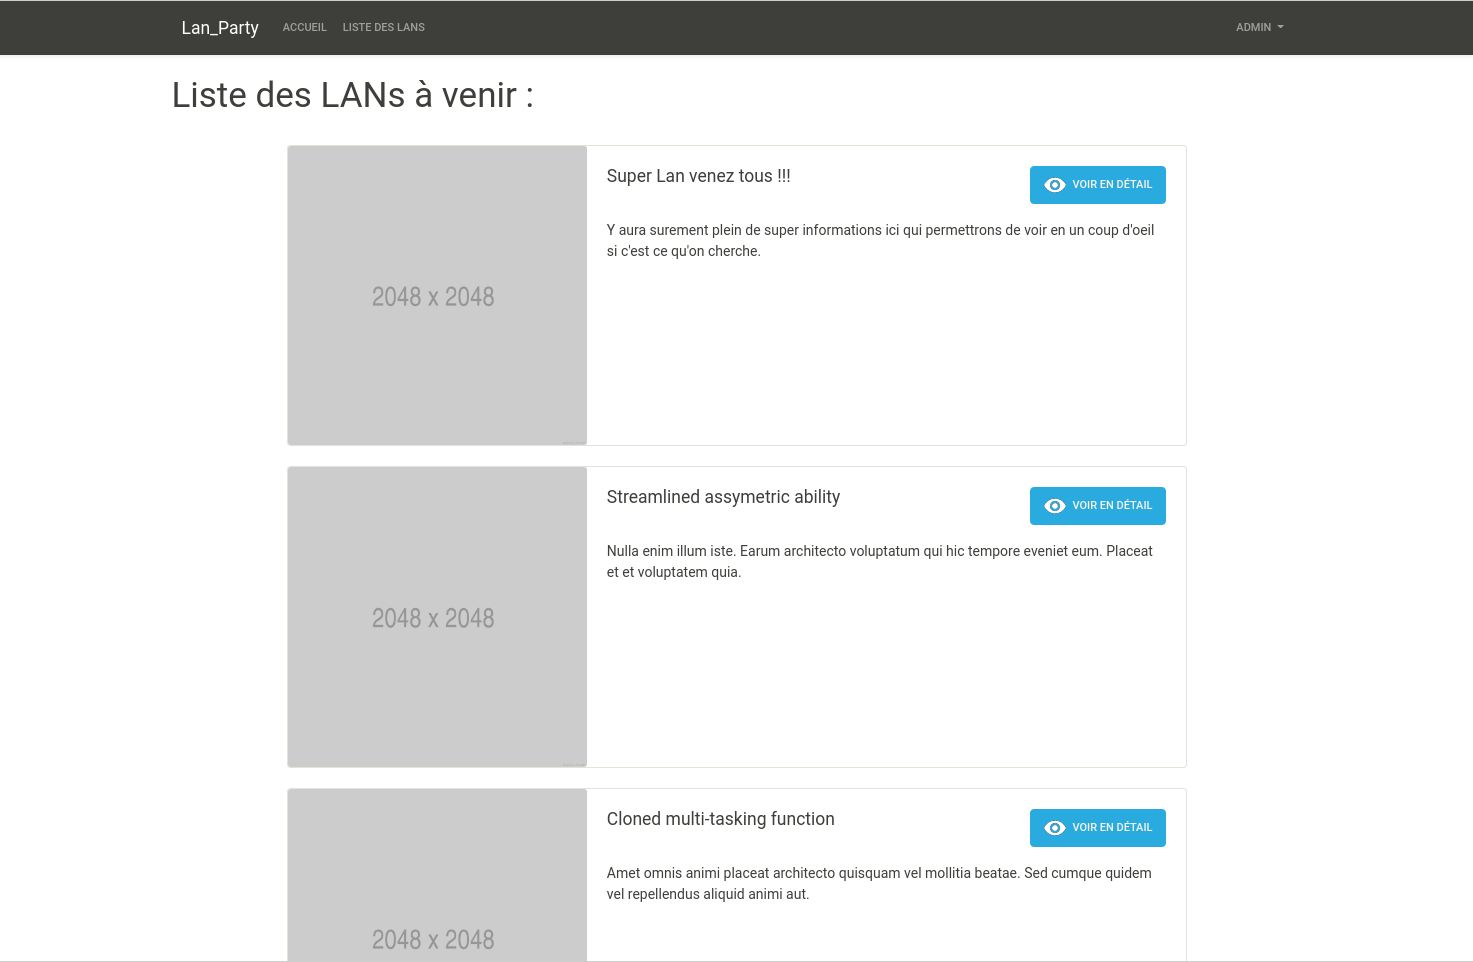
\includegraphics[scale=0.20]{images/liste.png}
\caption{Liste des Lans}
\label{}
\end{figure}

\begin{figure}[H]
\centering
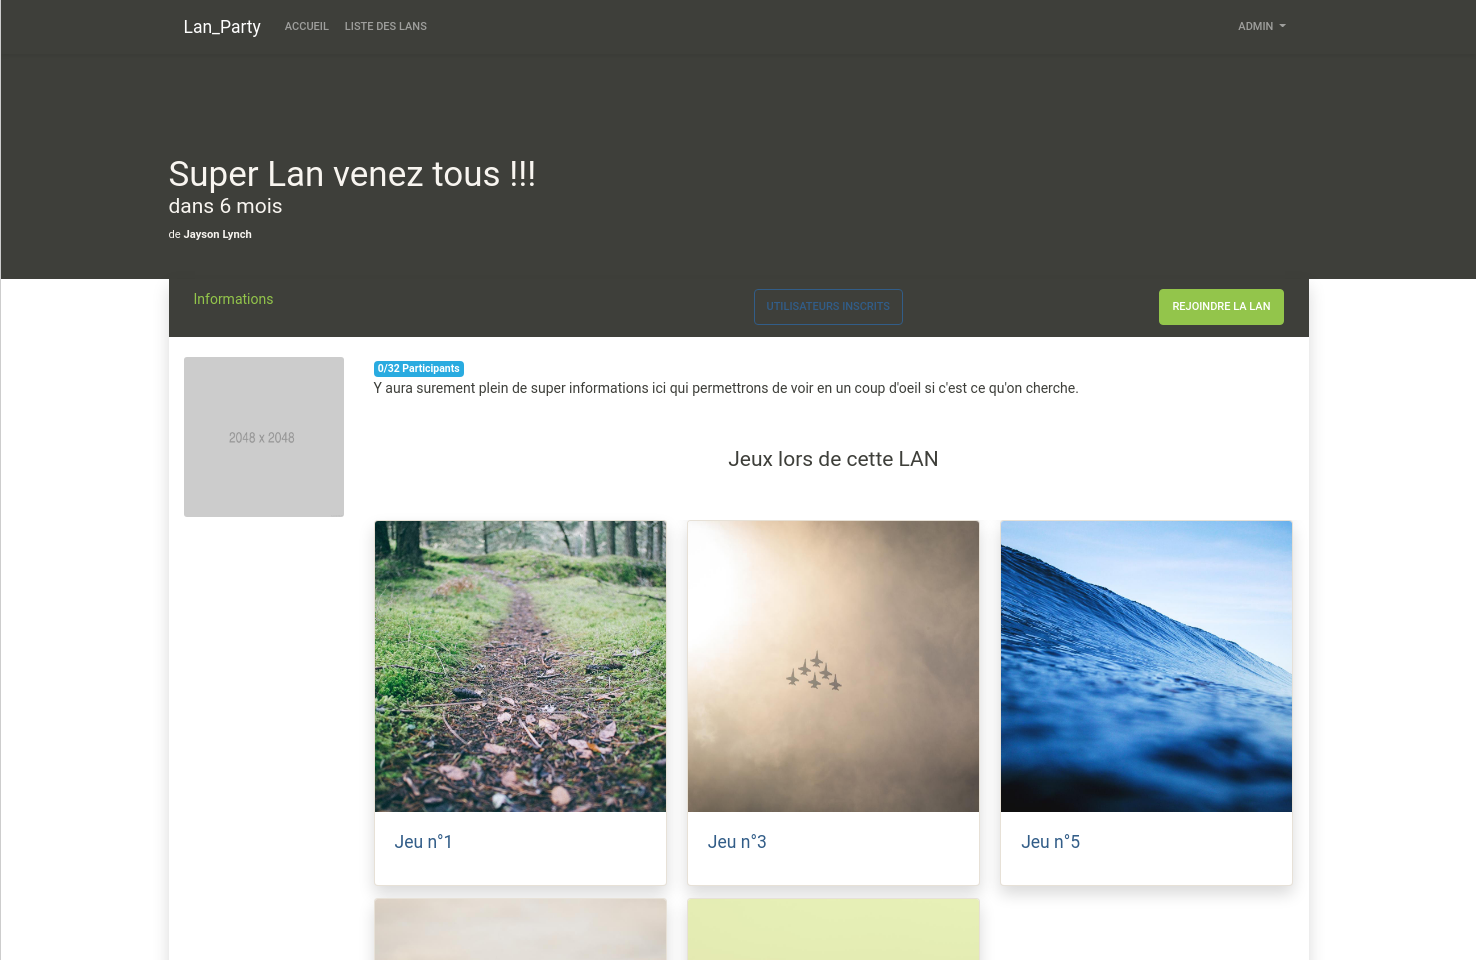
\includegraphics[scale=0.20]{images/fiche_lan.png}
\caption{Fiche d'une LAN}
\label{}
\end{figure}

\subsection{Partie Joueur}

Les joueurs ont accès à la possibilité de rejoindre une LAN depuis la fiche de celle-ci. De plus si le joueur s'est proposé comme aide pour l'organisation, il a accès à la liste des tâches qu'il lui a été affecté par les organisateurs.

\begin{figure}[H]
\centering
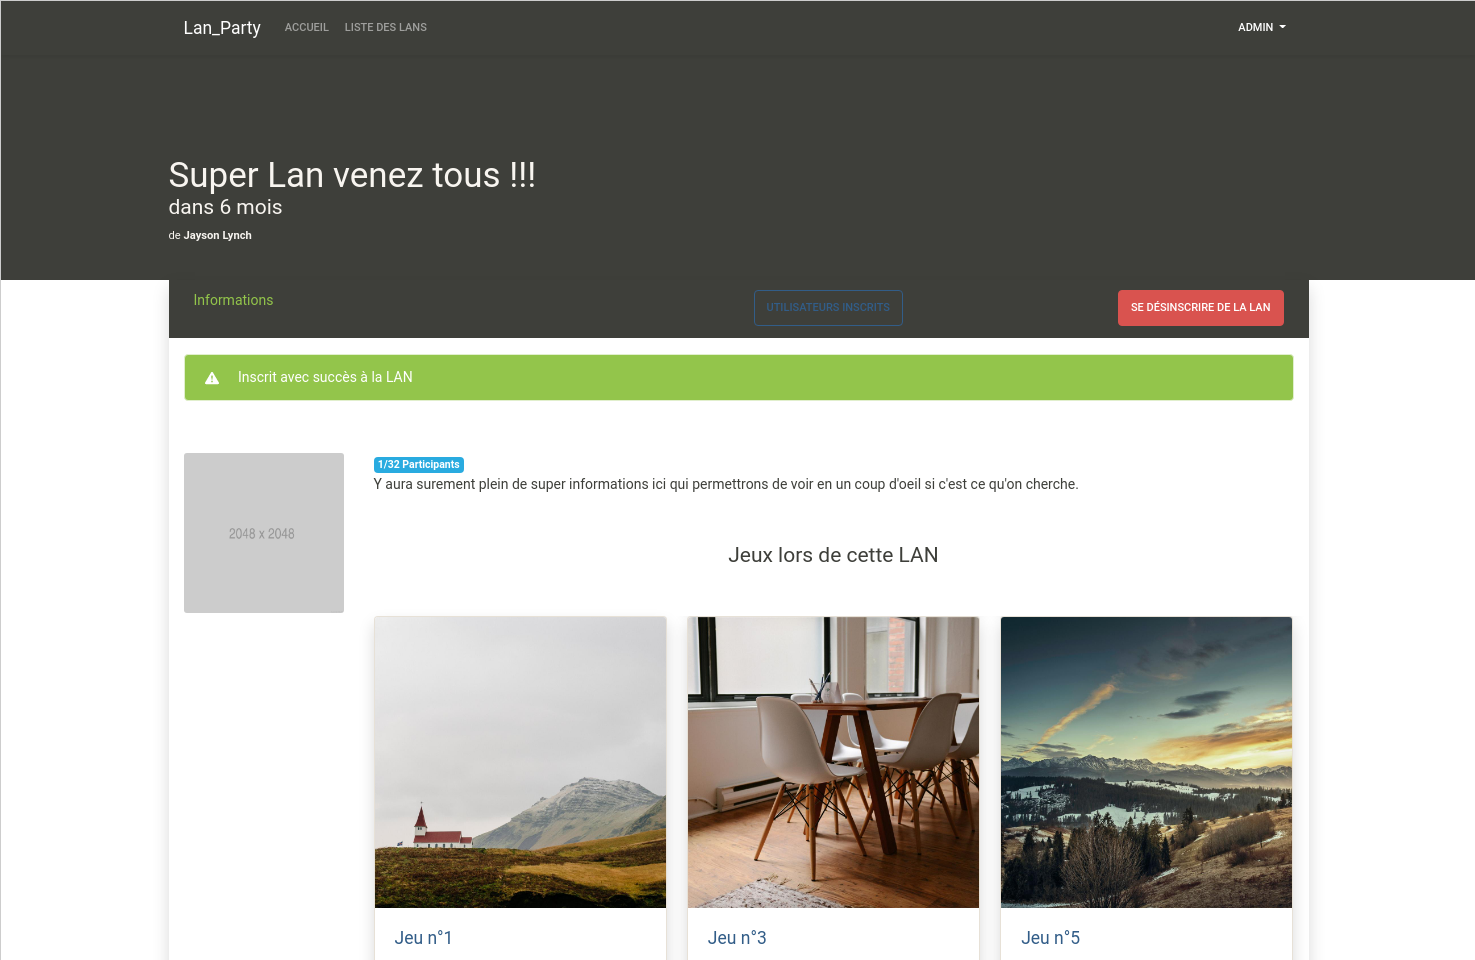
\includegraphics[scale=0.20]{images/inscrit.png}
\caption{Fiche d'une LAN après inscription}
\label{}
\end{figure}

\subsection{Partie Organisateur}

L'organisateur as accès au menu de gestion des LANs, permettant de les créer/modifier/supprimer et publier des LANs. La liste des LANs de l'organisateur contient donc aussi les LANs non publiées.

\begin{figure}[H]
\centering
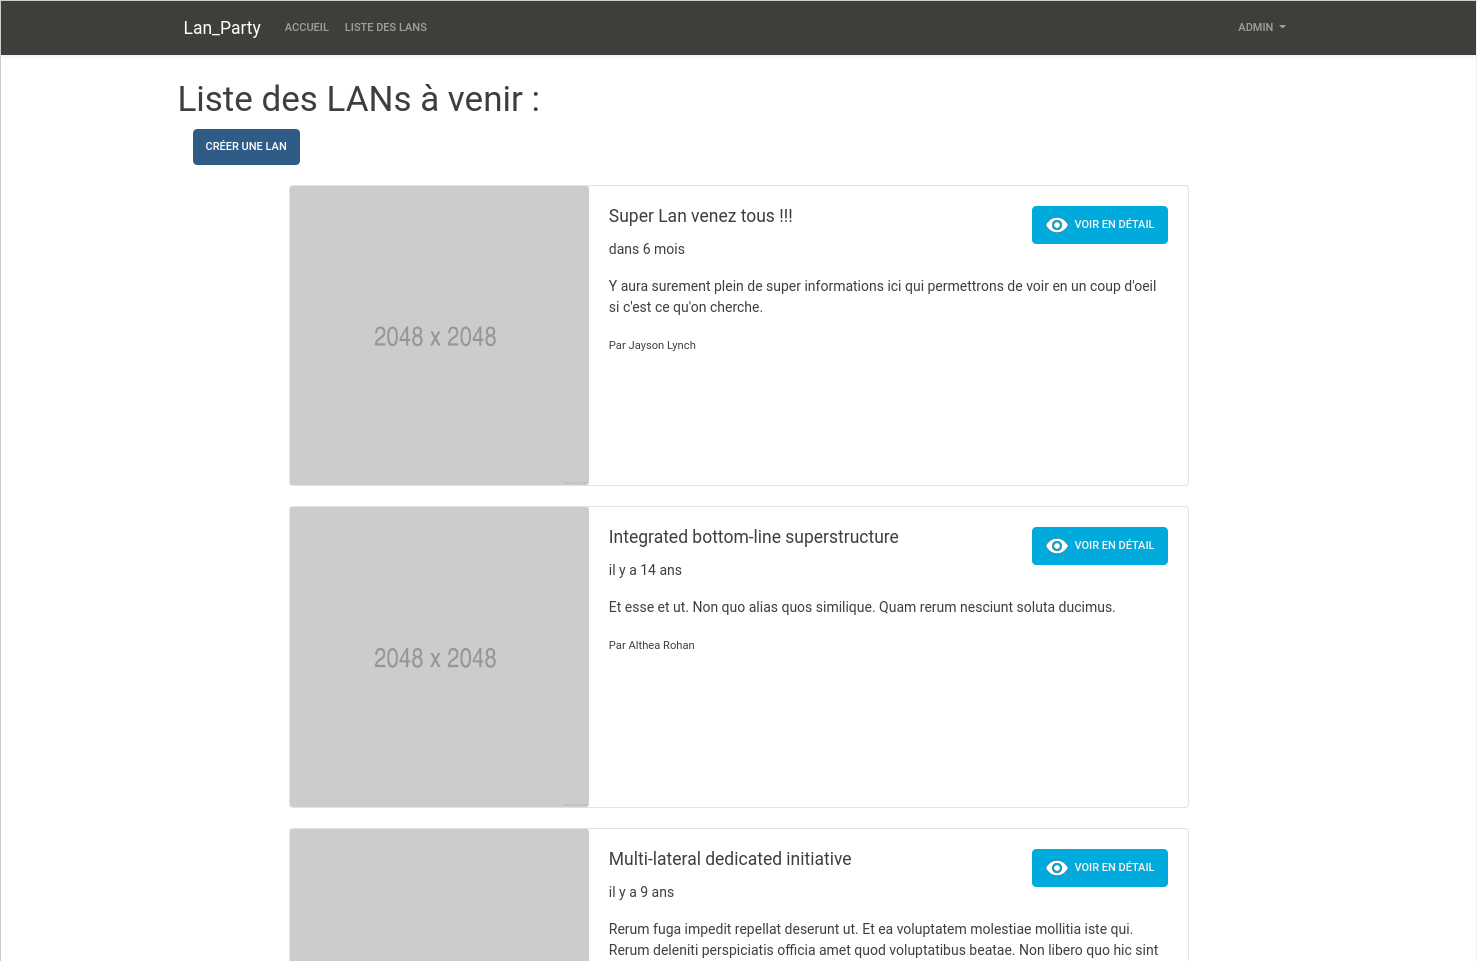
\includegraphics[scale=0.20]{images/liste_orga.png}
\caption{Liste des LANs en tant qu'organisateur}
\label{}
\end{figure}

L'organisateur peut choisir une "miniature" comme image, qui sera stockée dans le système de fichiers du serveur.

\subsection{Partie Tournoi}

La gestion des tournois est effectuée grâce à un site web externe, challonge.com, qui propose la gestion des arbres de tournois (rounds, déclaration de victoire/défaites, inscriptions...). En effet, ce site met à la disposition des utilisateurs une interface de programmation ou API pour ses utilisateurs.
Il a donc été choisi d'utiliser cet API. Pour éviter des problématiques de confidentialité et éviter les limites posées par le sites (nombre de requêtes maximum), notre application ne possède pas de clé et c'est l'organisateur qui devra se créer un compte challonge et rentrera sa clé dans notre application.
L'organisateur peut donc créer un tournoi s'il à un compte sur ce site. Grâce à sa clé d'api challonge, il peut lier son tournoi de l'application à challonge. Notre application en elle-même ne gère pas les tournois mais les relègue à challonge. Elle permet de gérer automatiquement les inscriptions désinscriptions à un tournoi et la génération des arbres sur le site. Aucun utilisateur n'aura besoin de se créer un compte, seulement l'organisateur et le(s) éventuel(s) administrateurs.


\subsection{Génération des données}

La base de données utilise les factories et les seeders de Laravel pour générer automatiquement un jeu de données de test. On a utilise la bibliothèque PHP Faker pour générer automatiquement des noms, des textes ou toute autre données que l'on pourra insérer dans la base de données.

Il a été plus compliqué de générer des relations (par exemple, les utilisateurs qui sont inscrits à une LAN), mais le seeder les génère aussi.

Pour les images factices, nous avons choisi d'utiliser le site placeholder.com qui met à disposition une image d'une seule couleur avec un texte prenant la taille que l'on veut, jusqu'à plus de 3000 pixels. Pour des images plus réalistes, on a pu utiliser le site picsum.photos qui propose des vraies images aléatoires de la résolution souhaitée.

\subsection{Amélioration possibles}

Il a été envisagé d'utiliser un autre site pour récupérer les noms de jeux déjà existant, ce qui permet à l'organisateur de chercher un jeu dans une base de données afin d'en récupérer toutes les informations nécessaires (images, nombre de joueurs, réseau, plage de ports, etc...). Mais la documentation n'était pas forcément à jour ni très précise sur l'utilisation par rapport à la version actuelle, et peu voir pas de ressources étaient présentes pour apprendre à l'utiliser. C'est pourquoi nous n'avons pas pu l'intégrer.

Nous avons pu grâce à différents outils (Bootstrap, jQuery) créer des vues réactives. Celles-çi sont de plus adaptées à la naviguation sur téléphone portable (responsive design grâce à Bootstrap) et il serait possible d'augmenter le dynamisme des pages web avec l'utilisation de JavaScript. Tout ce que l'on fait est possible avec des simples formulaires html/php, mais l'utilisation d'AJaX permet de rendre les formulaires plus réactifs avec plus de fluidité avec en contrepartie seulement un coût en calcul côté client, qui est cependant relativement léger, et donc qui n'aurait pas beaucoup altéré la naviguation sur téléphone, et un développement supplémentaire côté serveur, si nous avions eu le temps: En effet cela aurait nécessité le développement d'une API pour l'application, même si ce n'est pas obligatoire cela aurait été la choix optimal, ce que Laravel d'après la documentation peut sans doute permettre. Nous n'avons cependant pas eu l'occasion d'apprendre cette partie de Laravel, développant d'autres parties de la gestion de l'application.

\end{document}
